\documentclass[mathserif]{beamer}
\usetheme[secheader]{pecostalk}

\newcommand{\commentout}[1]{}

\newcommand{\cpp}[0]{\texttt{C++}}

\usepackage{accents}
\usepackage{amsfonts}
\usepackage{amsmath}
\usepackage{amssymb}
\usepackage{color}
\usepackage{mathtools}
\usepackage{subfigure}
\mathtoolsset{showonlyrefs,showmanualtags}

\definecolor{DarkGreen}{rgb}{0.13,0.55,0.13}


\setbeamercolor{block body}{bg=white}

\graphicspath{{./figs/ ../figs/}}

\date{23 January 2012}
\author{Jesse Chan, Nathan V. Roberts}
\institute{Center for Predictive Engineering and Computational Sciences \\
  Institute for Computational Engineering and Sciences \\
  The University of Texas at Austin
}
\title[Camellia + MPI]{
Extending Camellia: Distributed Stiffness Matrix Determination with MPI}
\begin{document}

\section{Status Update in Brief}

\begin{frame}
\titlepage
\end{frame}

\begin{frame}
\frametitle{Outline}
\tableofcontents
\end{frame}

\begin{frame}
\frametitle{What we had in September 2011}
Support for:
\begin{itemize}
\item meshes of arbitrary degree, with arbitrary combinations of triangles and quads
\item p-refinements
\item easy-to-specify bilinear forms
\item easy-to-specify inner products, {\bf including automatically specified mathematician's and optimal inner products}
\item rudimentary plotting of field variables using MATLAB
\item all computations done in serial
\end{itemize}
\end{frame}


\begin{frame}
\frametitle{What we've added}
Support for:
\begin{itemize}
\item h-refinements
\item automatic adaptivity
\item mesh-dependent inner products
\item better plotting of fields, plus simultaneous flux plotting, using MATLAB
\item {\bf distributed optimal test function and stiffness matrix determination using MPI}
\item next up/underway: work on 2D Burgers' equation (following MIT paper)
\end{itemize}
\end{frame}

\section{Extending Camellia for MPI}

\begin{frame}
\frametitle{Goals for Camellia+MPI}
Immediately (today):
\begin{itemize}
\item distributed optimal test function and stiffness matrix determination
\item perform timing experiments to measure speedup and determine where the serial bottlenecks are
\end{itemize}
Eventually (someday):
\begin{itemize}
\item parallel data structures for Mesh, Solution
\item parallel solver (MUMPS already works on Nate's laptop)
\end{itemize}
\end{frame}

\begin{frame}
\frametitle{Distributing Element Computations: Partitioning Strategy}
To take advantage of MPI, we need to partition the Mesh somehow.  What's a good way to do this?
\begin{itemize}
\item Key consideration in designing distributed algorithms: {\bf data locality} and {\bf minimizing inter-node communication}.
\item In FEM algorithms, data locality generally follows spatial locality---in DPG, we'll have information to communicate about fluxes and traces along each edge shared by two MPI nodes.
\item We use a Hilbert space-filling curve to determine a spatially-local partition of elements, using Trilinos's Zoltan package.
\end{itemize}
\end{frame}

\begin{frame}
\frametitle{Example Partitions}
%\begin{figure}[!htb]
%\center
%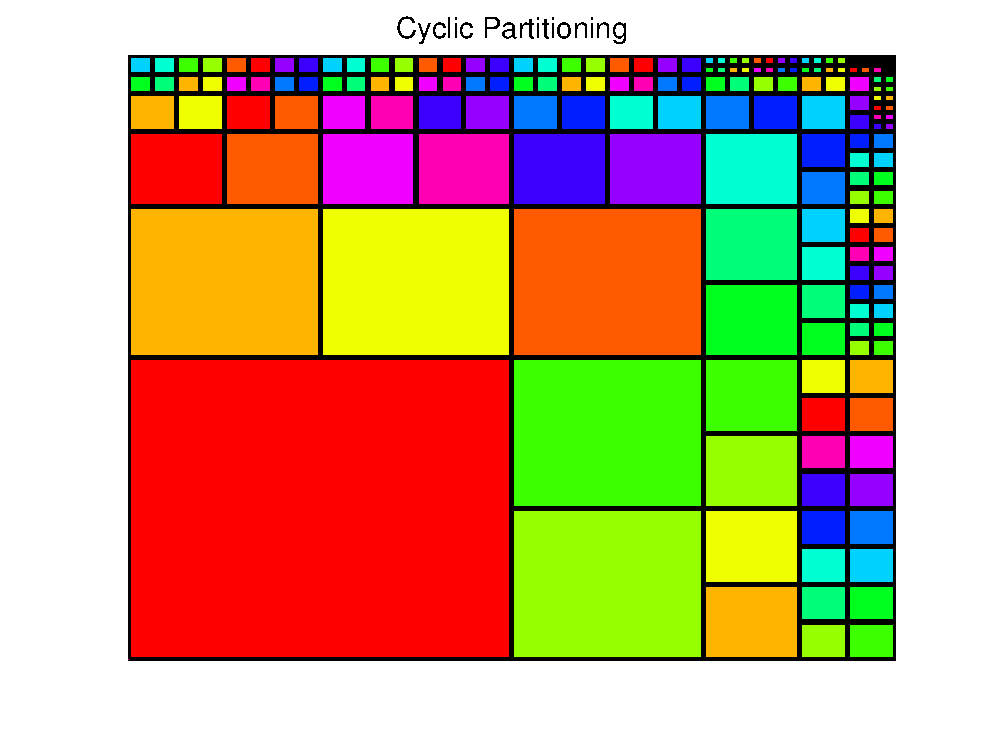
\includegraphics[scale=.38]{../figs/cyclic.pdf}
%\caption{}
%\end{figure}
\begin{columns}[c]
\begin{column}{5.5cm}
\begin{block}{``Cyclic'' partitioning}
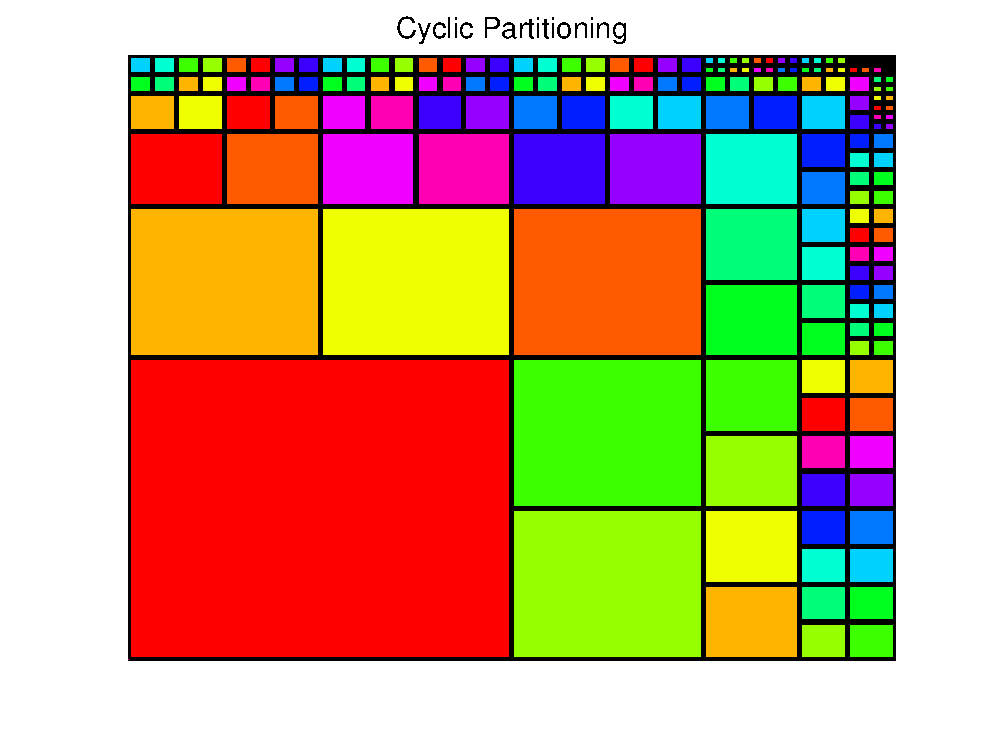
\includegraphics[width=5.5cm]{../figs/cyclic.pdf}
\end{block}
\end{column}
\begin{column}{5.5cm}
\begin{block}{Hilbert SFC partitioning}
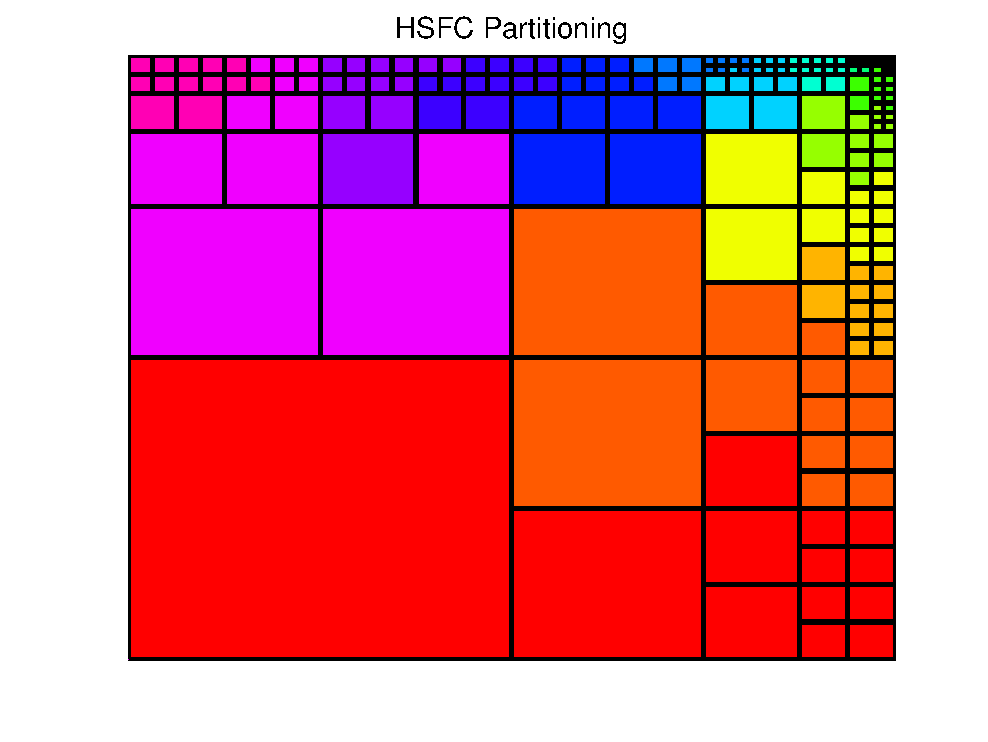
\includegraphics[width=5.5cm]{../figs/hsfc.pdf}
\end{block}
\end{column}
\end{columns}
\end{frame}

\begin{frame}
\frametitle{Details of Original Mesh Implementation: ElementType}
\begin{itemize}
\item The low-level methods used to do integration, etc. in Trilinos allow {\bf batching} of elements---i.e. computations can be done for several elements at once for better efficiency.
\item These methods assume that all elements in a batch are of like type.
\item Camellia's meshes have elements of different types.
\item Design goal: allow computations to be done on all elements that are of like type.
\end{itemize}

All of this motivates the introduction of the ElementType class.
\end{frame}

\begin{frame}
\frametitle{Details of Original Mesh Implementation: ElementType}
Camellia's ElementType is determined by the following features of the element:
\begin{itemize}
\item trial space (a \emph{DofOrdering} object),
\item test space (a \emph{DofOrdering} object),
\item element topology (a Trilinos \emph{CellTopology} object)
\end{itemize}

All elements of like type can be addressed as a batch.  Supporting this required the creation of a number of structures within Camellia's Mesh class that are indexed by ElementType.
\end{frame}

\begin{frame}
\frametitle{Two Element-Partitioning Mechanisms}
The division of the Mesh into elements of like ElementType can be thought of as a partitioning of the Mesh.  How should this interact with the partitioning provided by the HSFC?
\begin{itemize}
\item effectively, want a {\bf two-level} partition: first, apply HSFC, and then use ElementType within an MPI node for batching
\item this means that each of the Mesh's data structures indexed by ElementType should also be indexed by partitionNumber
\item unfortunately, we still need to support some mesh-global operations indexed by ElementType: thus we need to duplicate several of our lookups.
\item the eventual goal: get rid of those mesh-global operations, replacing them with distributed versions.
\end{itemize}
\end{frame}

\begin{frame}
\frametitle{Other Code Modifications}
Changes required outside of Mesh:
\begin{itemize}
\item introduce abstract MeshPartitionPolicy class, with concrete HSFC and Cyclic implementations
\item in Solution, determine dof partitioning, and supply that to the Epetra CrsMatrix
\item in Solution: after the solve, distribute solution coefficients to all nodes (will not be required once we have a  completely distributed implementation of all methods)
\end{itemize}
\end{frame}

\section{Timing Experiments}

\begin{frame}
\frametitle{Experimental Setup}
For a convection-dominated diffusion problem, we used four meshes of size varying from 202 elements to 12928 elements, and timed the overall computation, as well as the following individual components on each node:
\begin{itemize}
\item local stiffness matrix computation
\item global stiffness matrix assembly
\item solve
\end{itemize}
We ran this on Lonestar, using between 1 and 64 MPI nodes.  For a cleaner experiment, we only used 1 core from each machine.
\end{frame}

\begin{frame}
\frametitle{Strong Scaling}
Strong scaling: fix the problem size, and distribute the workload across increasing numbers of processors.
\begin{columns}[c]
\begin{column}{5.5cm}
\begin{block}{``Cyclic'' local stiffness computation}
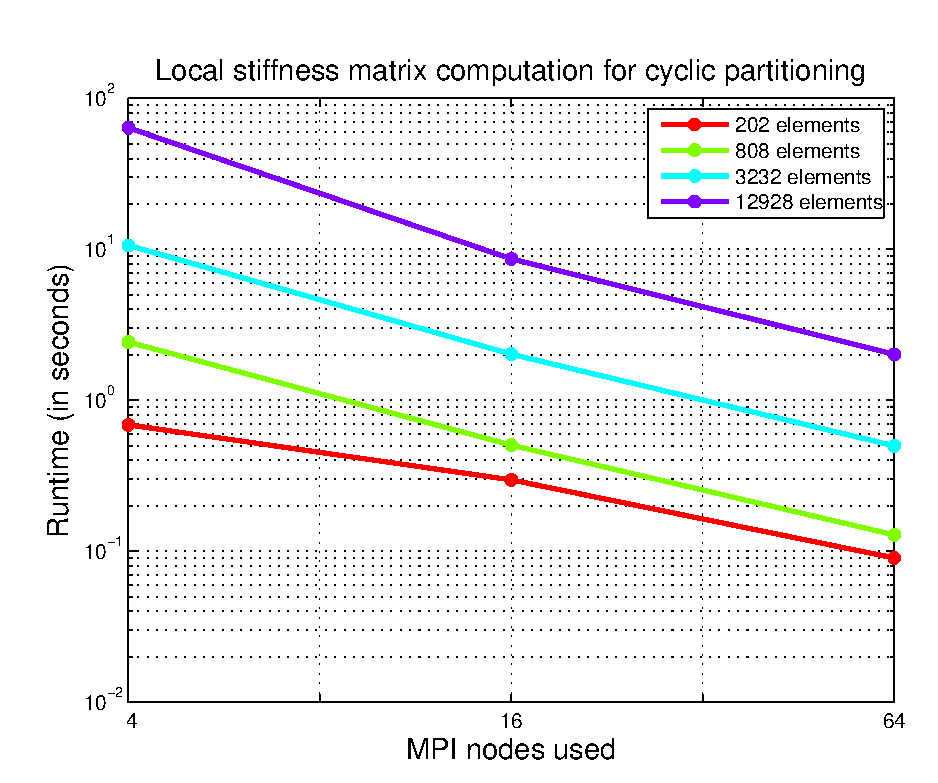
\includegraphics[width=5.5cm]{../figs/scalingFigs/cyclicStrongScalingLocal.pdf}
\end{block}
\end{column}
\begin{column}{5.5cm}
\begin{block}{Hilbert SFC local stiffness computation}
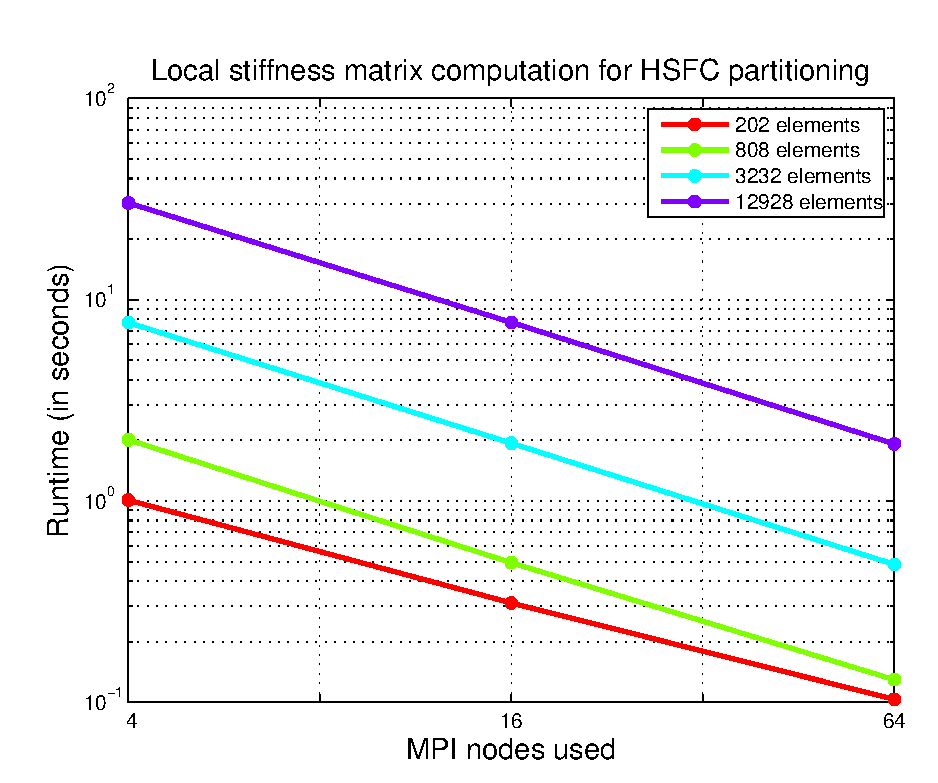
\includegraphics[width=5.5cm]{../figs/scalingFigs/hsfcStrongScalingLocal.pdf}
\end{block}
\end{column}
\end{columns}
\end{frame}


\begin{frame}
\frametitle{Strong Scaling, Global Assembly}
\begin{columns}[c]
\begin{column}{5.5cm}
\begin{block}{``Cyclic'' global assembly}
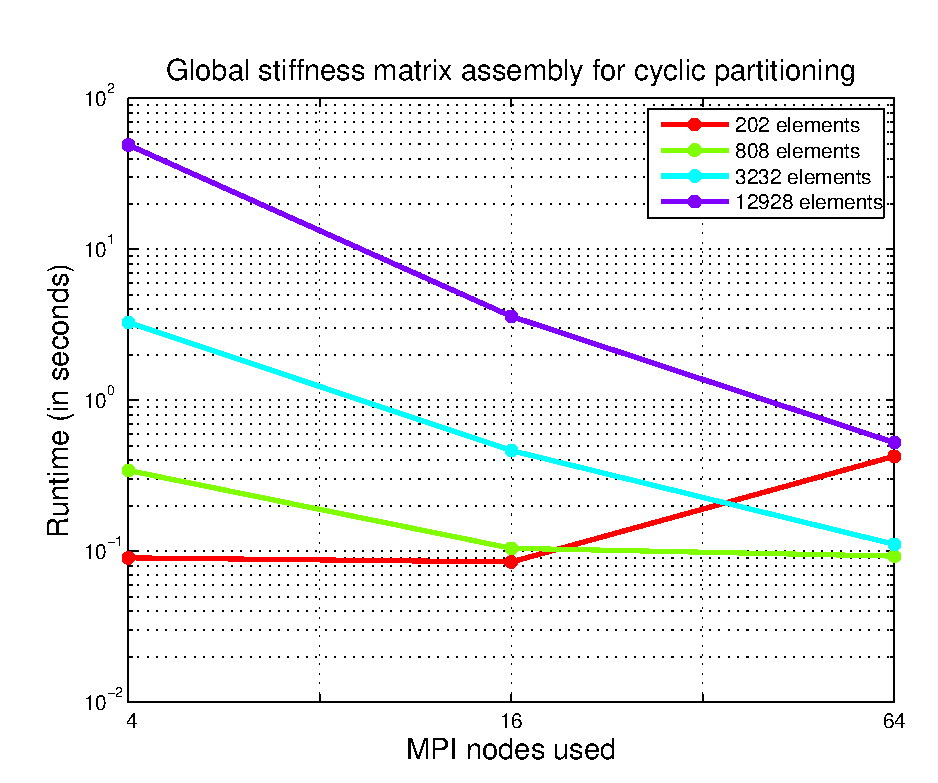
\includegraphics[width=5.5cm]{../figs/scalingFigs/cyclicStrongScalingAssembly.pdf}
\end{block}
\end{column}
\begin{column}{5.5cm}
\begin{block}{Hilbert SFC global assembly}
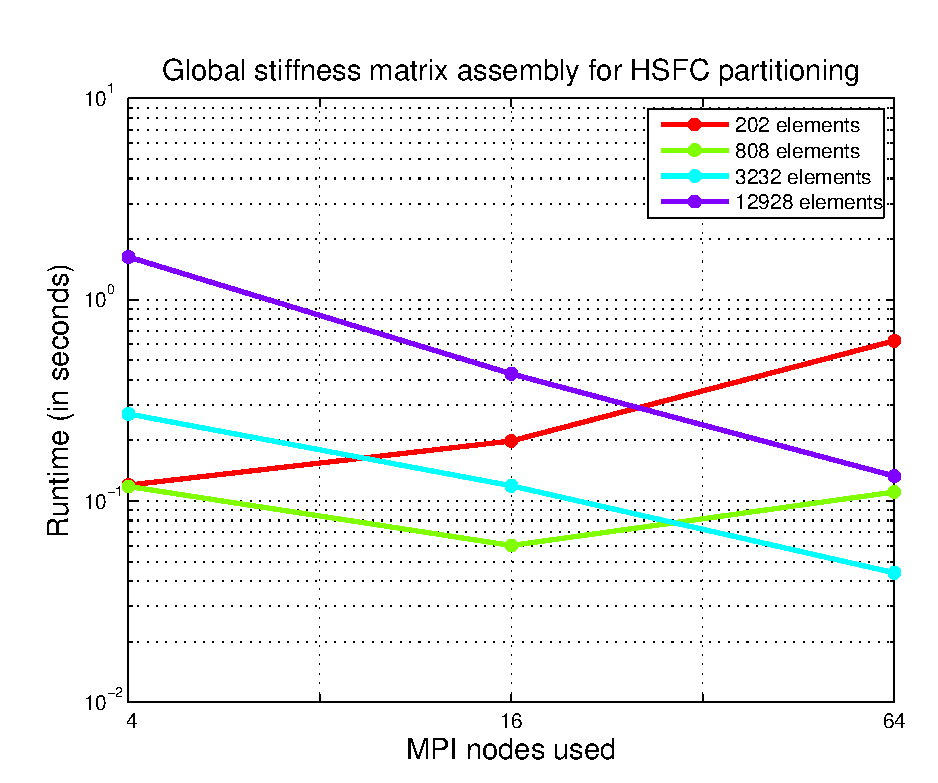
\includegraphics[width=5.5cm]{../figs/scalingFigs/hsfcStrongScalingAssembly.pdf}
\end{block}
\end{column}
\end{columns}
\end{frame}

\begin{frame}
\frametitle{Weak Scaling}
Weak scaling: fix the problem size per MPI node, and increase the number of MPI nodes.  Hope to see constant runtime.
\begin{columns}[c]
\begin{column}{5.5cm}
\begin{block}{Local Stiffness}
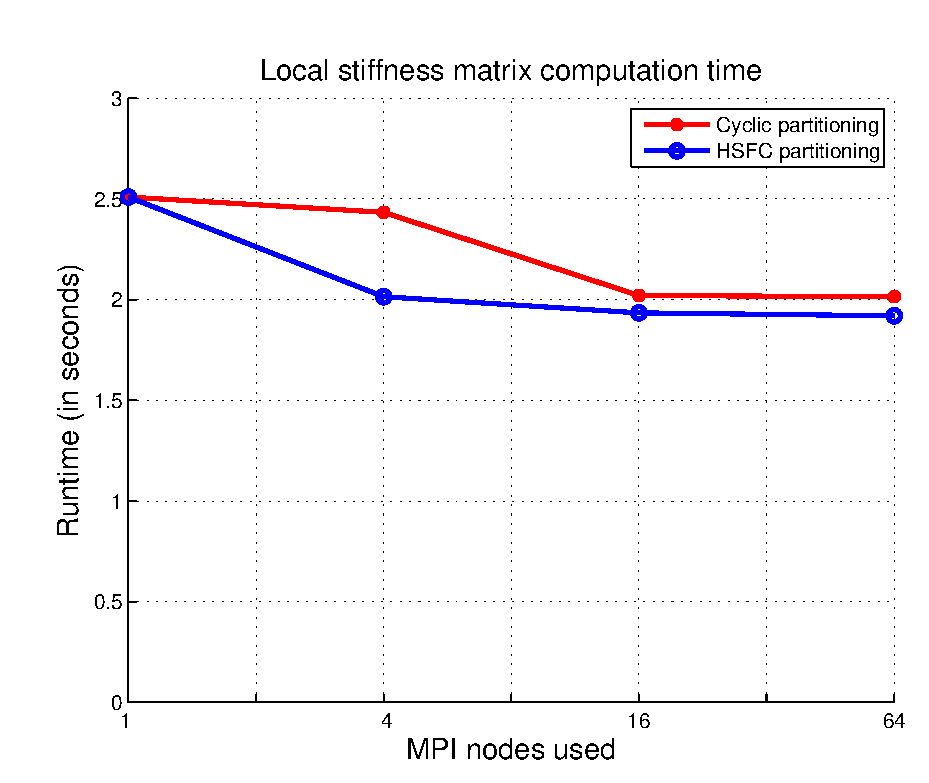
\includegraphics[width=5.5cm]{../figs/scalingFigs/weakScalingLocal.pdf}
\end{block}
\end{column}
\begin{column}{5.5cm}
\begin{block}{Global Assembly}
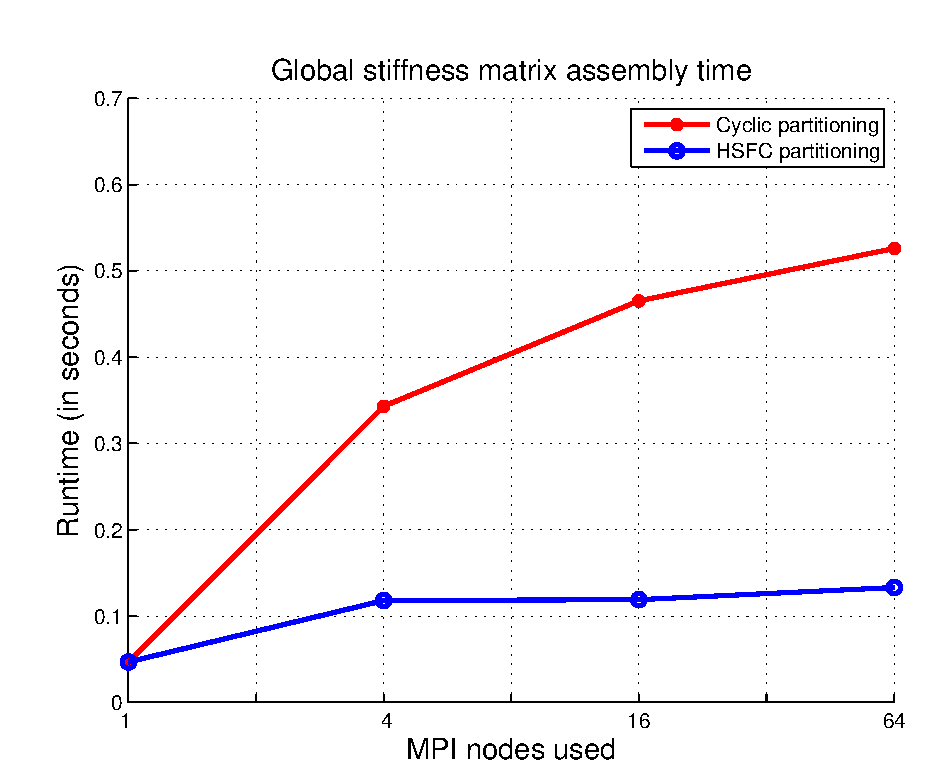
\includegraphics[width=5.5cm]{../figs/scalingFigs/weakScalingAssembly.pdf}
\end{block}
\end{column}
\end{columns}
\end{frame}

\begin{frame}
\frametitle{Total Runtime Analysis}
Examine the fraction of time spent in various computations as the number of MPI nodes increases.
\begin{columns}[c]
\begin{column}{5.5cm}
\begin{block}{202 elements, 13,343 does}
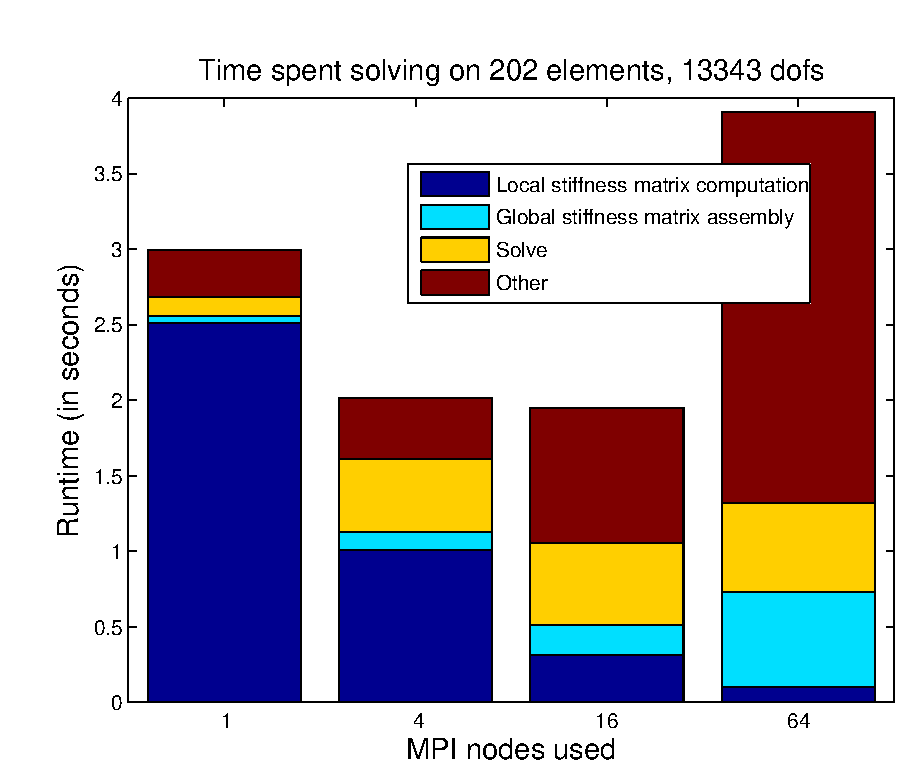
\includegraphics[width=5.5cm]{../figs/scalingFigs/bar_ref0.pdf}
\end{block}
\end{column}
\begin{column}{5.5cm}
\begin{block}{12,928 elements, 819,393 dofs}
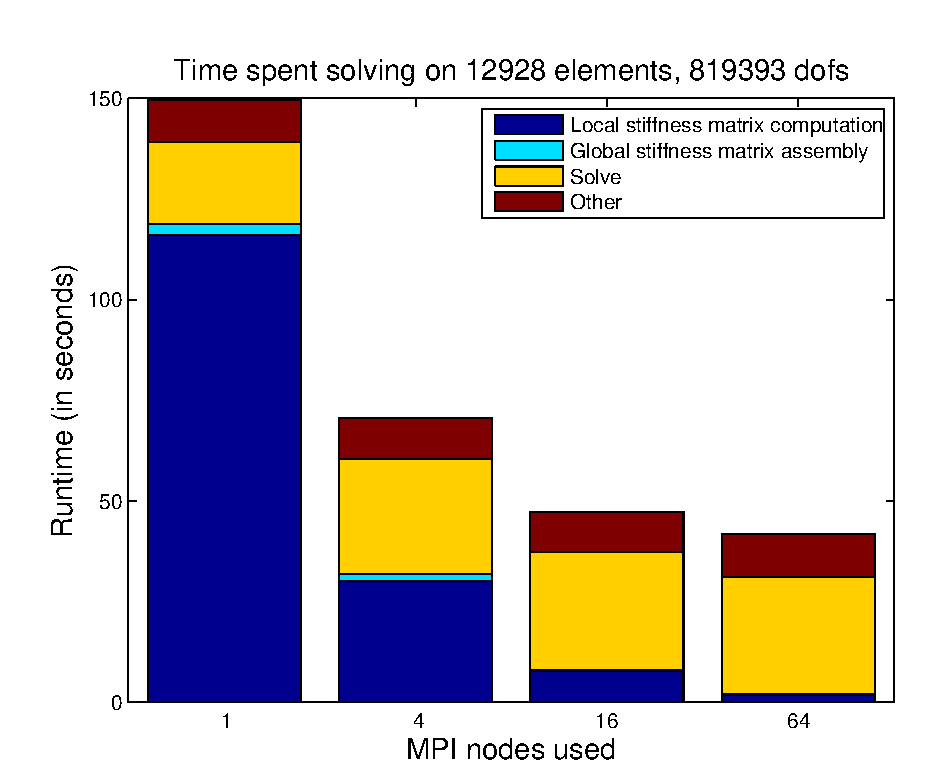
\includegraphics[width=5.5cm]{../figs/scalingFigs/bar_ref3.pdf}
\end{block}
\end{column}
\end{columns}
\end{frame}


\section{Parallel Adaptivity}

\frame{
\frametitle{Experiments with parallel adaptivity}
We have implemented Heuer and Demkowicz's inner product in Camellia
\[
\left((\tau,v),(\delta \tau ,\delta v)\right)_V=C(K,\epsilon)\|v\| + \epsilon\| \nabla v\| + \|\beta \cdot \nabla v \|_w + \|\tau \|_w + \|\nabla \cdot \tau \|_w 
\]
where $C(K,\epsilon) = \min(\epsilon,|J(K)|)$. 
\begin{figure}[!h]
\centering
\subfigure{
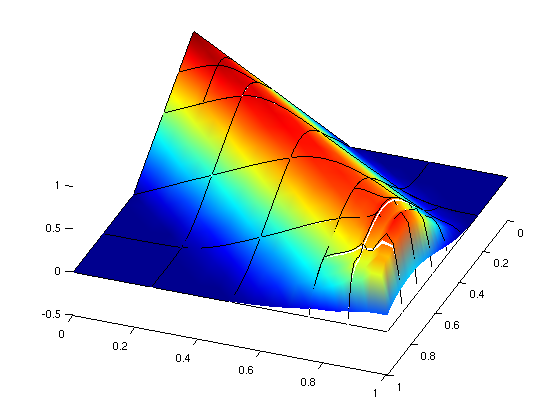
\includegraphics[scale=.3]{simplePlot.png}
}
\subfigure{
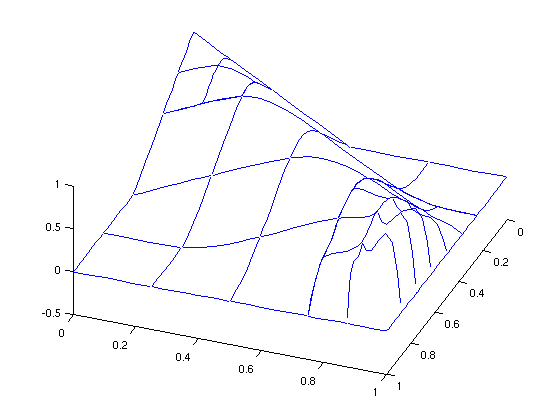
\includegraphics[scale=.3]{simpleFlux.png}
}
\end{figure}
}

\frame{
\frametitle{For better pictures, $\epsilon = 5e-2$, slightly skew advection.}

\begin{figure}[!h]
\centering
\subfigure{
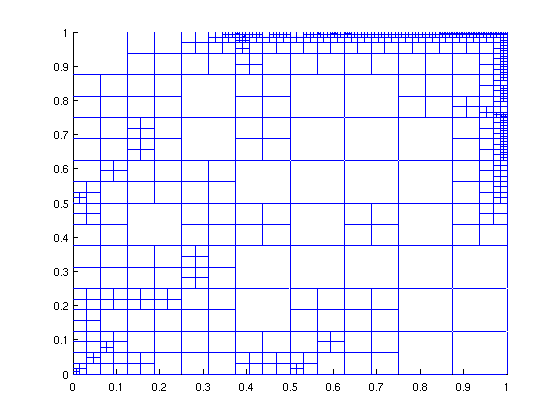
\includegraphics[scale=.25]{demoFlux.png}
}
\subfigure{
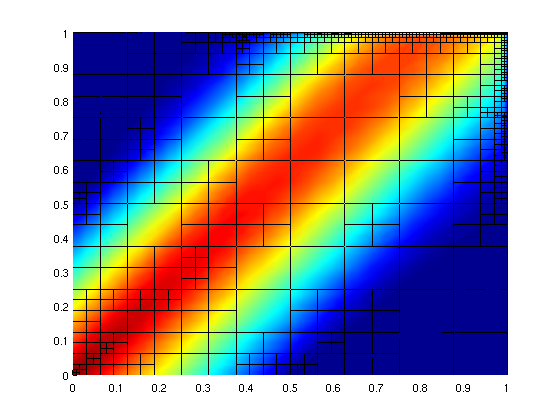
\includegraphics[scale=.25]{demoSolMesh.png}
}
\subfigure{
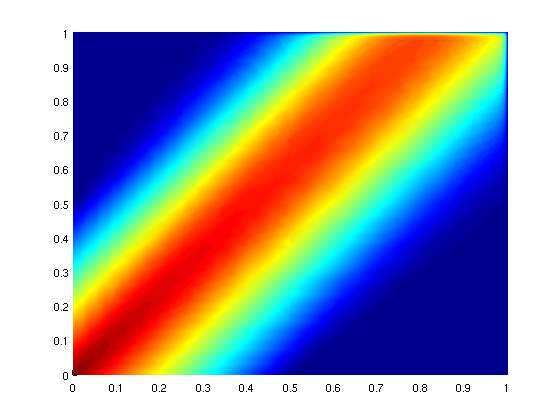
\includegraphics[scale=.25]{demoSol.png}
}
\end{figure}
}

\frame{
\frametitle{To make sure we still work at smaller scales, $\epsilon = 1e-3$}
\begin{figure}[!h]
\centering
\subfigure{
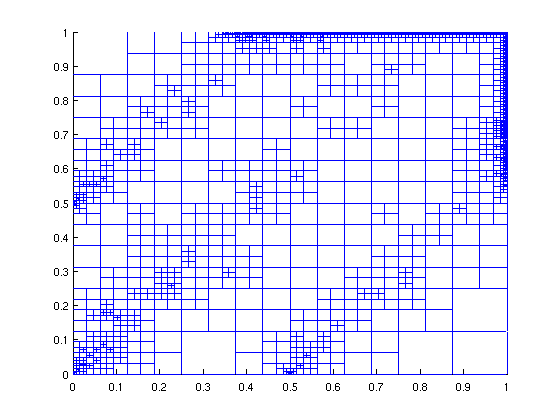
\includegraphics[scale=.35]{denseMesh.png}
}\subfigure{
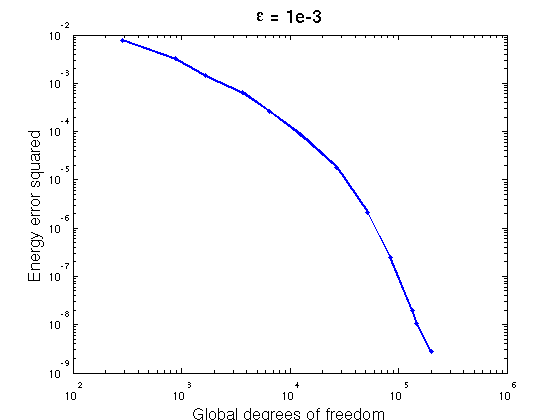
\includegraphics[scale=.35]{errorRate.png}
}
\end{figure}
}


\section{Future Work}
\begin{frame}
\frametitle{Future Work}
We are pretty satisfied, for now, with our parallel performance: we expect that we will be able to do our 2D Navier-Stokes simulations in reasonable time with the code as it stands.  But there is still significant opportunity to extend Camellia to solve larger problems still:
\begin{itemize}
\item distribute the solve using MUMPS or an iterative solver,
\item improve load balancing for meshes of variable polynomial order,
\item distribute mesh construction and storage, and
\item distribute solution storage.
\end{itemize}

\end{frame}

\begin{frame}
\begin{center}
  \vfill
  Thank you.
  \vfill
  Questions?
  \vfill
\end{center}
\end{frame}


\end{document}
